\documentclass[11pt,a4paper]{article}
\usepackage[margin=20mm]{geometry}
\usepackage{fontspec,graphicx,booktabs,longtable,array,amsmath,url}
\setmainfont{texgyretermes-regular.otf}[BoldFont=texgyretermes-bold.otf,ItalicFont=texgyretermes-italic.otf,BoldItalicFont=texgyretermes-bolditalic.otf]
\usepackage[hidelinks]{hyperref}
\title{Supplementary Material R2\\Exact GPU Traceback under a Memory Budget}
\author{Dabin Jeong\\Korea University\\cudabinary@korea.ac.kr}
\date{Run ID: \texttt{rtx4060ti\_wfa\_mechanism\_20261019}}
\begin{document}\maketitle
\section{Claims and reading guide}
This supplement accompanies the six-page English A4 manuscript. The contribution is a concrete block-local GPU realization of an existing reachability collector, with independent guarded arena capacity and measured whole-job tradeoffs. It is not a new garbage-collection principle, an automatic selector, or evidence that new hardware is necessary. Main performance and separately instrumented diagnostics use different binaries and are never pooled. All M units below mean $2^{20}$ eight-byte records, not decimal megabytes.

The corrected same-binary 20M/32 experiment has five fresh-process repetitions per mode. Both modes reserve 5,739,913,483~bytes (5,474.008~MiB); OFF takes 28.121~s and Full 24.320~s by median, a 13.5\% reduction, with 118 versus zero supported-pair CPU rescues. Against the lighter guarded path allowed an extra worker, benefits are smaller than the old large-arena-only comparison. The earlier 12.7\% result remains historical: exact outputs passed, but three inherited shared same-value writes remain in its frozen source, so absence of impact cannot be proved retrospectively. Its last diagnostic has an external-query STOPPED flag and is excluded from clean performance and primary causal evidence.

\subsection{Complete revised-source ONT table}
\begin{center}\small\setlength{\tabcolsep}{4.8pt}\begin{tabular}{lllrcrr}
\toprule
Cap (GiB) & Path & $C/w$ & Reserved (MiB) & Time median [min,max] (s) & $n$ & CPU rescues\\
\midrule
3.0 & Guarded no-GC & 10M/34 & 2,923.384 & 33.299 [32.590, 33.585] & 3 & 533\\
3.0 & Guarded no-GC & 10M/35 & 3,008.071 & 32.489 [31.350, 32.563] & 3 & 533\\
3.0 & GC binary OFF & 10M/34 & 3,008.384 & 31.655 [31.292, 31.897] & 3 & 533\\
3.0 & Full GC & 10M/34 & 3,008.384 & 26.797 [26.166, 27.007] & 3 & 0\\
5.5 & Guarded no-GC & 20M/32 & 5,314.008 & 27.561 [27.475, 28.583] & 3 & 118\\
5.5 & Guarded no-GC & 20M/33 & 5,478.696 & 27.608 [27.267, 28.422] & 3 & 118\\
5.5 & GC binary OFF & 20M/32 & 5,474.008 & 28.121 [27.460, 28.676] & 5 & 118\\
5.5 & Full GC & 20M/32 & 5,474.008 & 24.320 [23.790, 24.850] & 5 & 0\\
\midrule
--- & CPU BiWFA20 & --- & --- & 25.789 [25.008, 26.799] & 5 & ---\\
\bottomrule
\end{tabular}
\end{center}
\paragraph{Timing.} Whole-job time includes reading input, classifying and ordering pairs, preparing partitions, starting processes and contexts, allocating and initializing buffers, GPU work, CPU routing and exact rescue, synchronization, closing score and CIGAR output, and child exit. Common reference, configuration and ID loading, imports, reference generation, external validation and hashes are outside the clock. No fsync, cold-cache, fixed-clock or confidence-interval claim is made. Detailed traces and profilers are off in the main table; minimal allocation, status and fallback logging remains. Offline bounded configuration screens are reported separately, not disguised as a cost-free online selector.

\section{Input, contract and support}
The contract is exact global gap-affine: match 0, mismatch 2 and gap$(L)=3+L$, no band or heuristic. References check optimal score; the checker verifies positive full RLE CIGAR, actual M/X base semantics, I/D affine costs, and complete consumption of both sequences. Tied optimum strings may differ. Pair IDs are zero-based original-file indices, e.g. \texttt{50k:02647}. Pairing and orientation are never recombined.

The ONT 50k source has 10,000 pairs with maximum-length median 6,104~bp, 90th percentile 31,352~bp and maximum 49,993~bp. Of these, 9,112 have A/C/G/T and lengths below 32,768; 888 are length-routed to CPU. The unused short set has 4,488 pairs, excluding original 10k IDs 0--511. All 5,000 10k pairs also occur in 50k. Configuration screens use only the old selection, not the already inspected ONT confirmation. CCS is a separate read-technology/source dataset with no pair-content duplicates; it is not an independent donor study or an arrival trace. The 2,375-pair CCS confirmation was already seen before this round and is never called a fresh holdout.

\begin{center}\small\begin{tabular}{lll}\toprule
Input & Public source & Original SHA256 prefix\\\midrule
10k gzip & block-aligner v0.0.0 release & b338ec6baf884e8b\\
50k gzip & block-aligner v0.0.0 release & b8ccfc38d3a64660\\
CCS real archive & Zenodo 23118370 & 5231f89c219235f8\\
Normalized CCS & \texttt{rw\_ccs.seq} & fc543c4b2b0e566a\\\bottomrule\end{tabular}\end{center}
Full hashes, byte counts, original URLs and pair-ID lists are in the companion evidence/guide. The Zenodo metadata and publisher supplement describe HG002 mapped read--reference pairs; mapping/extraction versions and read-name correspondence are not available here. No new independent ONT corpus is claimed.

\paragraph{Representation checks.} Signed 16-bit offsets limit each GPU sequence to 32,767. The fixed scoring uses five rolling slots. $E=16,384$ and the tested smaller bounds keep diagonal/offset and fixed-array requirements within the audited path; guard capacity remains below 32-bit index limits and allocation arithmetic uses corrected size\_t expressions. Source-bound or step exhaustion is distinguished from an arena guard, collector error, result-chain error and actual cudaMalloc failure. There is no observed device OOM in the completed comparisons. Unsupported symbols are CPU-routed unchanged; no wildcard or normalization semantics are introduced.

\section{Byte model and comparison implementations}
Let $q=\operatorname{align4}_{+}(5(2E+1))$, where strict source padding is $\operatorname{align4}_{+}(x)=x+4-(x\bmod4)$. For $N$ GPU pairs, $b=\min(B,N)$ and actual-order maximum unpacked/packed batch bytes $U,P$, the tracked successful-path reservation is
\begin{align*}
M={}&8Cw+30qw+M_{GC}\\
 &+8\lfloor E/8\rfloor b+68b+40N+U+P+11,\\
M_{GC}={}&8w\lceil C/32\rceil\quad\hbox{(GC binary, even mode 0)}.
\end{align*}
The guarded binary has no bitmap/rank term. $C$ is clamped to the source bound $(2E+1)\lfloor E/8\rfloor$. The model matches logged primary reservation byte-for-byte. Driver/context/module internals, host/pinned storage, physical residency and paging are excluded. Reclamation does not release the CUDA arena. The main budgets are 3/5.5~GiB reservation caps; detailed diagnostics use a separate 6.75~GiB cap and an extra 8,344~bytes per eligible pair (76,030,528~bytes total). Diagnostic reservation must not be quoted as primary reservation.

The common software includes clean metadata, padding/size fixes, allocation reuse, skipped unnecessary arena clears and current exact WFA2 ultralow rescue. GPU unsupported routing uses 16 CPU threads; rescue uses four, with overlap. Worker count is a block-pool setting, not measured residency. Guarded and GC register limits are 64/96; actual compiled resources and hashes are retained in build logs. Same-binary mode 0/1 holds those resources and allocated scratch constant, but changes continued GPU work, CPU restart and pipeline overlap.

\subsection{Bounded CPU screens on old selection}
\begin{center}\small\begin{tabular}{lrlrrl}\toprule
Mode & Threads & Order & Time(s) & Peak RSS(MiB) & Outcome\\\midrule
ultralow & 20 & desc & 6.053 & 357.8 & Exact pass\\
high & 20 & raw & --- & 10,826.7 & Signal11 (under AS cap)\\
high & 4 & raw & --- & 11,900.0 & Signal11 (under AS cap)\\
low & 20 & raw & 55.877 & 7,313.4 & Exact pass\\
med & 20 & raw & 50.559 & 9,325.1 & Exact pass\\
single & 4 & raw & 14.572 & 6,505.6 & Exact pass\\
ultralow & 20 & desc & 5.890 & 355.5 & Exact pass\\
ultralow & 20 & raw & 5.764 & 363.7 & Exact pass\\
\bottomrule\end{tabular}\end{center}

Each row is one selection screen, except the two separately retained descending BiWFA checks. A 12~GiB process address-space cap protects the host. The two high-mode signal 11 failures are excluded from performance selection; their elapsed times are not throughputs. They do not alone distinguish physical OOM, failed allocation handling or another implementation failure. One prescribed lower-thread check also fails. Med/low and Singletrack complete exact outputs but lose this selection screen. Current Singletrack at four threads is a feasible measured alternative, not evidence that every thread count was optimized. CPU affinity and exhaustive host-memory tuning remain untested.

\subsection{Smaller execution bounds}
\begin{center}\small\begin{tabular}{lrrrrrr}\toprule
Path & $E$ & $w$ & Effective C(M) & Reserved MiB & Time(s) & Rescues\\\midrule
Full & 4096 & 64 & 4.000488 & 2,213.332 & 13.177 & 333\\
Full & 8192 & 40 & 16.000977 & 5,402.141 & 12.886 & 85\\
Guarded & 4096 & 64 & 4.000488 & 2,149.324 & 14.078 & 333\\
Guarded & 8192 & 40 & 16.000977 & 5,242.131 & 11.991 & 85\\
\bottomrule\end{tabular}\end{center}

These are single old-selection screens, with equal bounded opportunities per GPU family. Requested C is 20M, but source clamping gives 4.000488M at E4096 and 16.000977M at E8192. The selected E8192 settings are repeated on the full input: guarded 32.333[30.691,32.402]s and Full 31.725[30.012,32.331]s, with 384 supported-pair CPU rescues each, plus the 888 unsupported pairs. Reducing E preserves final exactness through rescue; it changes GPU work distribution. We do not claim exhaustive optimality of the 64/40-worker screen settings.

\subsection{Refreshed short/CCS fixed settings}
\begin{center}\small\begin{tabular}{llrrr}\toprule
Input & Choice & Reserved MiB & Median[min,max](s) & Rescues\\\midrule
Short ONT & BiWFA20 & --- & 1.037 [1.013,1.072] & ---\\
Short ONT & Full 2M/64 & 1,374.681 & 1.348 [1.346,1.474] & 0\\
Short ONT & Guarded 4M/64 & 2,366.681 & 1.455 [1.334,1.648] & 0\\
CCS & BiWFA20 & --- & 0.569 [0.549,0.576] & ---\\
CCS & Full 20M/32 & 5,455.420 & 2.618 [2.354,2.629] & 0\\
CCS & Guarded 4M/64 & 2,373.428 & 3.430 [3.243,3.439] & 38\\
\bottomrule\end{tabular}\end{center}

These 18 jobs refresh the previously fixed three choices per dataset after the shared-writer fix. The amendment was recorded before these requests. No setting is tuned from this refresh; CCS remains seen confirmation. Short GPU timing ranges overlap and CPU is faster. CPU also wins on CCS, despite GC improving the tested GPU path. These revised numbers replace, rather than pool with, the historical short/CCS timings in the main manuscript.

\section{Root preservation and qualification}
At score s the fixed recurrence reads M(s--2),M(s--4),I/D(s--1). At the collection boundary all five M/I/D slots are conservative stored roots spanning ages 0--4; partial vectors remain in their arrays. Recurrence-local references are quiescent at the common block barrier and future updates read remapped pointers. Backward predecessor links and a complete root closure are required. Stable rank is injective and never moves a record forward. Per tile, all source payloads/links are loaded before stores, with barriers before the next tile; later unread tiles cannot be damaged. This is a conditional code-specific preservation argument, not universal CUDA memory-model certification.

The common fix assigns only cursor initialization and two shared exist=false groups to tid0. Thread-local distance, steps and ring index continue on all threads; existing barriers remain. Independent reviewers checked the exact diff, source dependencies and source versions. Actual-helper unit tests verify payload/link/root remapping, partial-vector preservation, NULL and shared ancestry, bitmap 31/32/33, compact-tile 255/256/257 and rank-tile 8191/8192/8193 boundaries. The first 33 cases include duplicate NULL styles; they are not 33 distinct graph shapes. An extended 96 worker-case test uses two disjoint blocks and three collections including append in the new namespace after remapping, H=1 and invalid-offset poison pointers.

Independent DP 160 pairs per guarded/off/on path verifies 480 pair-outputs but calls no GC. The separate helper tests call 354 collections (66+288). Public full-CIGAR diagnostics exercise repeated real collection. Negative-k/global-offset helper-unit boundaries, prefix mode, arbitrary penalties and corrupt-DAG expected-failure tests remain outside this helper matrix. Production paths still have independent pointer/result checks. Passing finite tests is not universal race freedom.

Compute Sanitizer reports WDDM debugger-interface initialization failure and Device not supported. Memcheck returns 0 while printing ERROR SUMMARY 2; racecheck returns 11 with the setup failure. Neither is a pass, and the two setup messages are not kernel-specific race findings. Initcheck/synccheck were not repeated after interface unavailability. Failed harness compile/include setup and the accidental guarded GC-prefix setup request are retained separately from successful alignment tests.

\begin{figure}[ht]\centering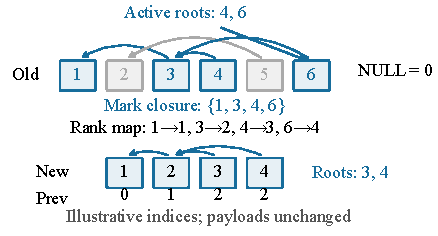
\includegraphics[width=.63\textwidth]{figures/gc_address_map.pdf}
\caption{Illustrative stable relocation, not a measured workload or memory curve.}\end{figure}

\section{Measured generation, retention and collection cost}
\begin{center}\small\begin{tabular}{lrrrrr}\toprule
C/w & Collected pairs & Calls & Max calls & Median live(\%) & Max retained(M)\\\midrule
10/34 & 788 & 1331 & 8 & 20.01 & 4.799\\
20/32 & 235 & 277 & 3 & 15.87 & 4.855\\
\bottomrule\end{tabular}\end{center}

Both Full 10 and Full 20 successfully generate 19,939,875,345 offloaded records across 9,112 pairs. Total reclaimed records are 7,933,518,117 and 3,643,079,979 respectively. These are cumulative logical counts across pairs/time, not simultaneously resident or freed device bytes. For each successful pair, generated = final occupied + sum(occupied-before minus retained-after). The direct counter agrees with this identity; event overflow/underflow flags are zero. The counter adds observed occupied increases and resets its baseline after successful GC. Failed no-GC append attempts beyond the guard are clamped to actually stored records, not called successful generation.

The max-retained statistic is only over collection events. It is neither the continuously sampled peak nor the minimum exact-traceback requirement. A final occupied count can exceed the last retained count because more records are appended before reaching the target.

\subsection{Named original-input witness}
The posthoc stress witness is \texttt{50k:02647}, lengths 32,390/31,912, optimum 14,823. It is selected by most GC calls among Full 10 pairs whose same-C guarded control fails capacity, then pair-ID tie break. It is not a typical-pair estimate. It generates 41,171,770 records in a 10M arena, collects eight times, and ends with 5,806,419 occupied records. Full CIGAR and complete consumption pass; the matched no-GC path uses exact CPU rescue.
\begin{center}\small\begin{tabular}{lrrrr}\toprule
Score & Generated(M) & Occupied before(M) & Retained(M) & Free after(M)\\\midrule
6482 & 7.502 & 7.502 & 1.137 & 8.863\\
8811 & 13.866 & 7.501 & 1.991 & 8.009\\
10415 & 19.377 & 7.503 & 2.684 & 7.316\\
11637 & 24.194 & 7.501 & 3.261 & 6.739\\
12615 & 28.433 & 7.500 & 3.748 & 6.252\\
13422 & 32.190 & 7.505 & 4.162 & 5.838\\
14101 & 35.531 & 7.502 & 4.508 & 5.492\\
14683 & 38.526 & 7.503 & 4.799 & 5.201\\
\bottomrule\end{tabular}\end{center}

Free-after excludes NULL but includes no claim about future generation. Full 20's collection-event retained/occupied median is 15.87\%; Full 10's is 20.01\%. The whole-input event distributions, rather than only this chosen witness, appear in the main figure. Posthoc length/optimal-score bins and pair-level counts are exported separately. Optimal score is explanatory oracle information, never a free prelaunch routing feature.

\subsection{Phase observations, not wall fractions}
\begin{center}\small\begin{tabular}{lrr}\toprule
Phase / interval & 10M/34 & 20M/32\\\midrule
Clear (cycles) & 85,047 & 169,523\\
Mark (cycles) & 50,348,618 & 77,465,816\\
Rank (cycles) & 1,830,438 & 3,563,530\\
Compact (cycles) & 104,597,296 & 208,868,861\\
Remap (cycles) & 2,568,103 & 3,422,459\\
Device span (ms) & 58.032 & 109.118\\
\bottomrule\end{tabular}\end{center}

Phase values are median per-call clock64 intervals; span is the median per-call device globaltimer interval. The compact phase includes scanning IDs, staged loads, synchronization and moved-link writes; the remap phase updates roots. Individual synchronization cost is not isolated. Trace overhead is present. Different workers overlap; summing intervals or dividing their sums by job wall time would be invalid. The 10M/34 and 20M/32 comparisons also change capacity and worker pool, so their job difference is not a pure GC-overhead measurement.

\section{Host completion and the avoided restart path}
\begin{center}\small\begin{tabular}{lrrrrr}\toprule
Mode & Routed ready(s) & Last rescue(s) & Last GPU visible(s) & All ready(s) & Job end(s)\\\midrule
OFF & 17.625 & 22.322 & 29.331 & 29.333 & 29.450\\
Full & 16.367 & --- & 25.549 & 25.550 & 25.695\\
\bottomrule\end{tabular}\end{center}

Times above are host CLOCK\_MONOTONIC observations relative to a bracketed parent origin. GPU-visible means the host has synchronized and received the last batch's results, not a bridged device timestamp. ``Ready'' is completed alignment/RLE in memory, before final output close and child exit. The extra CPU timestamp binary is diagnostic-only. Device globaltimer and host clocks remain separate raw fields.

\begin{center}\small\begin{tabular}{lrrrr}\toprule
Mode & Batch & Capacity rescues & CUDA bracket(s) & CPU callback(s)\\\midrule
OFF & 0 & 108 & 8.148 & 10.815\\
OFF & 1 & 10 & 5.229 & 0.977\\
Full & 0 & 0 & 10.649 & 0.063\\
Full & 1 & 0 & 4.986 & 0.027\\
\bottomrule\end{tabular}\end{center}

The OFF 118 failures occur in the first two batches (108+10), a distribution also present in primary status files. CPU callback 0 can delay batch 2 even while batch 1 overlaps the callback. Full finishes more GPU work and removes the CPU re-alignment path. This supports an execution-path mechanism, not additive decomposition of the whole-job gap. The last rescue is earlier than overall completion; one last rescue pair cannot explain the whole delay. Output/teardown intervals and the final normal RLE remain real work.

\section{Closest work and unclaimed scope}
\begin{center}\small\begin{tabular}{>{\raggedright\arraybackslash}p{.19\textwidth}>{\raggedright\arraybackslash}p{.34\textwidth}>{\raggedright\arraybackslash}p{.36\textwidth}}\toprule
Prior work & Existing method & Added/tested scope here\\\midrule
WFA2-lib 6176f947 & Active-root ancestor mark/rank/compact/remap and retained prefixes. See wavefront\_backtrace\_buffer.c:358,376,457. & Fixed private GPU arenas, block-local bitmap/rank and staged in-place tiles; the reachability principle is prior art.\\
WFA-GPU ff981ad0 & Persistent blocks, compressed history, E/worker/thread controls and CPU rescue. & Independent C guard, active collection and matched budget/completion ablation; baseline padding/reset/reuse fixes are shared.\\
BiWFA & Bidirectional breakpoint decomposition and recursive recomputation for exact low space. & Current ultralow CPU/rescue implementation is run, not hypothetically combined with GC.\\
Singletrack 7185195 & Reduced affine state with limited I/D reconstruction. & Current feasible four-thread exact CPU screen; a GPU fusion is unimplemented/unmeasured.\\
Khatri et al. 2026 & Footprint/concurrency and traceback envelopes, CPU memory-mode/thread fairness. & We implement and measure active-root GPU reuse with liveness and same-binary controls; the original characterization is not our novelty.\\\bottomrule\end{tabular}\end{center}

The characterization article is published online 14 October 2026, DOI 10.1080/17445760.2026.2745067, pp.1--42, International Journal of Parallel, Emergent and Distributed Systems. Official Crossref and publisher supplement 34493070 verify this; volume/issue were unavailable. We read its 29-page official supplement and metadata, not the inaccessible full main article. Dataset Zenodo 23118370 is cited separately. Singletrack's journal record is Bioinformatics 42(5):btag183, DOI 10.1093/bioinformatics/btag183. The inspected supplement already discusses E fallback, traceback capacity/concurrency, index limits and fair CPU baselines. No priority for that problem observation is claimed.

Shared arenas, dependency-minimized roots, GPU Singletrack, arbitrary penalties, prefix qualification, exhaustive CPU modes/affinity and additional independent ONT traces are not measured alternatives. Good fixed configurations remain the result; automatic selection is future work. The next useful step is a frozen evaluation on a provenance-clear independent ONT read--reference corpus, measuring whether the generation/retained-closure gap and rescue effect generalize before developing a selector.

miniWFA, wfalm and TALCO also appear in the characterization supplement but are not executed here. They remain outside this finite comparison, so the measured controls do not establish superiority over every exact alignment implementation.

\subsection{Historical large-arena grid and selector record}
The following is the prior frozen kernel generation, not revised-source performance. Its shared-writer hazards remain unresolved retrospectively. The inherited current-WFA2 rescue path is retained, but none of these times is pooled with the new table or used as a new-source SOTA comparison. Each row has three repetitions on the same 10,000 ONT pairs and E16384.
\begin{center}\small\begin{tabular}{llrrr}\toprule
Old path & C/w & Reserved MiB & Median(s) & Rescues\\\midrule
Guarded & 40M/16 & 5,239.004 & 34.718 & 0\\
Guarded & 32M/20 & 5,257.755 & 29.135 & 20\\
Guarded & 32M/21 & 5,518.443 & 28.951 & 20\\
Guarded & 40M/17 & 5,563.692 & 33.974 & 0\\
Guarded & 40M/21 & 6,862.443 & 29.547 & 0\\
Full & 20M/32 & 5,474.008 & 24.549 & 0\\
Full & 20M/40 & 6,831.510 & 25.653 & 0\\
\bottomrule\end{tabular}\end{center}

The old 32M/20 and 40M/16 arenas both total 5,120~MiB; their overall reservations differ from Full 20M/32. This is why equal arena storage was never equated to equal total memory. The prior selector design and negative results remain in historical/PRIOR\_REPORT\_ko.md and PRIOR\_POLICY\_DESIGN.md, alongside original receipts and their source identity. No selector is executed or proposed as this manuscript's method. Original raw projects remain preserved at the paths in those receipts; the historical receipt copy is not a new validation of those old binaries.

\section{Artifact map and exact replay boundary}
The named local archive is \nolinkurl{ICEIC2027_WFA_R2_Research_Package.zip}. Its guide is \texttt{REPRODUCE.md}; the experiment contains corrected and diagnostic source archives, exact binary/library hashes, settings, ID/reference files, full scores/CIGAR/status/trace outputs and failure receipts. Duplicate partition seq files are kept in native WSL and omitted from the portable mirror with byte/SHA256 reconstruction receipts; original public inputs are not silently discarded or recombined. Full source archives include added headers, not only a tracked-file patch.

Use the reproduction guide to separate receipt-only verification from CPU tests, build and GPU replay. Replays use a fresh output ID and the shared execution lock; existing sealed records are never overwritten. The 72 job receipts include two failed CPU screens, 39 primary long-input jobs, 18 scope refreshes, three diagnostics and remaining selection screens. Primary long-input outputs total 390,000 repeated checks, not independent pairs. The local delivery is not a public repository, DOI or submission. Original projects and the previous paper remain read-only; no paid cloud or publication action was performed.
\end{document}
